\documentclass{cernatsnote}

\usepackage{amsmath}
\usepackage{amssymb}

\title{Disease detection with machine learning}
\author{
	Manik Dawar, Pranav Kulkarni
}

\date{\today}

\begin{document}
\maketitle


\begin{abstract}
This lab report presents a comprehensive analysis of Fourier-transform infrared (FTIR) spectroscopy data derived from simulated case-control studies of individuals with lung cancer. Utilizing machine learning methodologies, including Logistic Regression and Support Vector Machines (SVM), we developed binary classifiers capable of distinguishing between cancerous and non-cancerous cases based on their infrared fingerprints. We achieve a AUC(area under the curve) of 0.90 with logistic regression versus 0.89 with SVM. Our results demonstrate the potential of FTIR spectroscopy and machine learning for disease diagnostics.
\end{abstract}



\\ \\ \\ 

\begingroup
\color{black}
\tableofcontents
\listoffigures 
\endgroup


\pagebreak

\section{Introduction}
Advancements in omics analyses of human biofluids have opened up new opportunities for disease diagnostics. Fourier-transform infrared (FTIR) spectroscopy, in particular, has emerged as a potent tool to investigate the molecular species within a sample simultaneously. In this experiment, we leverage FTIR spectroscopy to analyze the infrared fingerprints of serum samples from a simulated case-control study. This study comprises individuals with different solid tumors and carefully matched non-symptomatic reference individuals. By employing machine learning methodologies such as Logistic Regression and Support Vector Machines (SVM), we aim to classify these cases and controls effectively, offering valuable insights for disease diagnostics.





\section{Conceptual Background}
\subsection{Fourier Transform Infrared Spectroscopy (FTIR)}

Fourier Transform Infrared (FTIR) Spectroscopy is a powerful method of analysis used in the fields of chemistry, physics, and materials science. It is based on the principle of molecular vibrational spectroscopy, where infrared radiation is absorbed by molecules and induces vibrational excitation \cite{griffiths2007fourier}. Key concepts of FTIR spectroscopy:

\begin{enumerate}
\item \textbf{Infrared Spectroscopy:} Infrared spectroscopy pertains to the interactions between a molecule and radiation in the infrared region. These interactions can induce a change in the vibrational states of the molecule, producing a unique spectrum that can be used to identify the molecule or analyze its structure.

\item \textbf{Fourier Transform:} Fourier Transform is a mathematical tool used to convert a time-domain signal into its frequency-domain equivalent, and vice versa. In the context of FTIR, a Fourier transform is applied to the raw data (an interferogram) to obtain the desired spectral information.

\item \textbf{Molecular Vibrations:} Molecules can undergo various vibrational modes, such as stretching and bending. Each of these vibrational modes corresponds to a particular energy level. When a molecule absorbs infrared radiation, it transitions between these energy levels. The frequency at which these transitions occur is unique to each molecule, giving rise to the characteristic absorption spectrum.

\item \textbf{Interferometry:} The Michelson interferometer, typically used in FTIR, produces an interference pattern that varies with the difference in path length between its two arms. This pattern, or interferogram, is the raw data which is converted into the spectrum by the Fourier Transform.

\item \textbf{Advantages of FTIR:} Some of the key advantages of FTIR over dispersive IR spectroscopy include its superior speed, sensitivity, and resolution. FTIR can also directly measure all wavelengths simultaneously (the Fellgett’s or multiplex advantage), and the Signal-to-Noise ratio improves by the square root of the number of scans (the Jacquinot’s or throughput advantage).
\end{enumerate}

\subsection{Support Vector Machines}
Support Vector Machines (SVMs) are a set of powerful supervised learning algorithms used for classification and regression. They are particularly effective in high dimensional spaces and are versatile in modeling complex decision boundaries \cite{hearst1998support, bishop2006pattern}. 

The fundamental principle of SVMs is to construct a hyperplane as the decision boundary in such a way that the margin between two classes in the feature space is maximized. 

\subsubsection{Linear SVMs}
In the simplest case of a linear binary classifier, given a labeled training dataset where the labels are either +1 or -1, the SVM tries to find a hyperplane defined by \(w^T x + b = 0\) that separates the two classes. Here, \(w\) is the weight vector and \(b\) is the bias term. 

The decision rule for a new instance \(x'\) is given by:

\[
f(x') = \text{sign}(w^T x' + b)
\]

The optimal hyperplane that separates the two classes maximizes the distance (margin) to the closest points from each class. These closest points are called support vectors.

For a given hyperplane, the distance of a point \(x_i\) to the hyperplane is \( \frac{|w^T x_i + b|}{||w||_2} \). Therefore, the margin \(M\) can be defined as:

\[
M = \frac{1}{||w||_2}
\]

The optimization problem therefore becomes:

\[
\text{minimize} \quad \frac{1}{2} ||w||^2
\]
\[
\text{subject to} \quad y_i(w^T x_i + b) \geq 1, \quad \forall i
\]

This is a quadratic programming problem which can be solved using methods such as Sequential Minimal Optimization (SMO).

\subsubsection{Non-linear SVMs}
For non-linearly separable data, SVMs use the kernel trick. The kernel trick involves mapping the input features into a higher-dimensional space where a hyperplane can be used to separate the data. The decision function becomes:

\[
f(x') = \text{sign}\left(\sum_{i=1}^{N} \alpha_i y_i K(x_i, x') + b\right)
\]

Here, \(K(x_i, x')\) is a kernel function, which computes the inner product of the transformed vectors in the high-dimensional space, and \(\alpha_i\) are the Lagrange multipliers obtained from solving the dual form of the optimization problem. 

Common choices of the kernel function include the linear, polynomial, and radial basis function (RBF) kernels. The choice of kernel and its parameters depends on the problem at hand and is usually determined through cross-validation.





\subsection{Logistic Regression}

Logistic Regression is a statistical model used for binary classification problems. While it is a regression algorithm, it is primarily used for classification tasks \cite{hosmer2013applied, bishop2006pattern}.

The main idea of logistic regression is to find the probability of a certain event occurrence based on a set of features. Logistic regression predicts the probability of the target variable being true based on the input variables.

Mathematically, in a binary logistic regression model, the dependent variable is a binary variable that contains data coded as 1 (yes, success, etc.) or 0 (no, failure, etc.). In other words, the logistic regression model predicts \( P(Y=1) \) as a function of \( X \).

The logistic regression function \( p(X) \) is given by:

\[
p(X) = \frac{e^{\beta_0 + \beta_1 X}}{1 + e^{\beta_0 + \beta_1 X}}
\]

\noindent
Where:\\
- \( p(X) \) is the probability of the target (output) variable equals 1.\\
- \( e \) is the base of the natural logarithm (approximately equal to 2.71828).\\
- \( \beta_0 \) and \( \beta_1 \) are the parameters of the model.\\
- \( X \) is the input variable (feature).\\

The right-hand side of the equation can be simplified to:

\[
p(X) = \frac{1}{1 + e^{-(\beta_0 + \beta_1 X)}}
\]

This is known as the logistic function or the sigmoid function. Its output is a value between 0 and 1 which can be interpreted as the probability of the occurrence of an event.

The parameters \( \beta_0 \) and \( \beta_1 \) are estimated using maximum likelihood estimation. This involves finding the values of the parameters that maximize the likelihood of the observed data.

Logistic regression can be extended to handle multi-class classification tasks with the use of techniques like one-vs-all (also known as one-vs-rest) or one-vs-one.


\subsection{Confusion Matrix}

A confusion matrix, also known as an error matrix, is a specific table layout that is widely used for understanding the performance of a classification model. It illustrates the performance of an algorithm by displaying the correct and incorrect predictions in a tabular form \cite{powers2011evaluation}.

The confusion matrix for a binary classification problem is a 2x2 matrix with the following layout:

\[
\begin{array}{cc|c|c|}
 & & \multicolumn{2}{c}{\text{Predicted Class}} \\
 & & \text{Positive} & \text{Negative} \\
\hline
\multirow{\rotatebox[origin=c]{90}{\text{Actual Class}}} & \text{Positive} & \text{True Positives (TP)} & \text{False Negatives (FN)} \\
 & \text{Negative} & \text{False Positives (FP)} & \text{True Negatives (TN)} \\
\hline
\end{array}
\]

Here, 
- True Positives (TP) and True Negatives (TN) are the correctly predicted positive and negative instances, respectively.
- False Positives (FP) are the negative instances incorrectly predicted as positive.
- False Negatives (FN) are the positive instances incorrectly predicted as negative.

\subsection{Receiver Operating Characteristic (ROC) Curve}

The Receiver Operating Characteristic (ROC) curve is a graphical plot that illustrates the performance of a binary classifier as its discrimination threshold is varied. The ROC curve is created by plotting the True Positive Rate (TPR) against the False Positive Rate (FPR) at various threshold settings \cite{fawcett2006introduction, powers2011evaluation}.

The area under the ROC curve, known as the AUC-ROC, is a measure of the classifier's ability to distinguish between the classes. An AUC-ROC score of 1.0 indicates a perfect classifier, while an AUC-ROC score of 0.5 indicates a random classifier.

\subsection{Comparison of Confusion Matrix and ROC Curve}

While both the confusion matrix and the ROC curve are used for evaluating the performance of a classification model, the ROC curve provides a more comprehensive and generalized evaluation \cite{powers2011evaluation}.

The confusion matrix provides an absolute measure of the correct and incorrect classifications. However, it does not account for the different costs of different types of errors (i.e., the cost of false positives versus false negatives), and it does not provide any information about the trade-off between the sensitivity (TPR) and specificity (1-FPR).

On the other hand, the ROC curve visualizes the trade-off between sensitivity and specificity for all possible thresholds, not just a single cut-off point. This allows for a more nuanced understanding of the classifier's performance across a range of scenarios, making it a more general approach.

Moreover, by considering the area under the ROC curve (AUC-ROC), we get a single metric that summarizes the overall performance of the classifier across all thresholds, making it easier to compare different classifiers.












\section{Implementation of the code}


\subsection{Importing and structuring data}

The code for this section is contained in the file import\_data.ipynb. Our data processing workflow included the following steps:

\begin{enumerate}

\item \textbf{Importing Necessary Libraries:}
We began by importing several Python libraries essential to our work:

\begin{itemize}
\item \texttt{json}: This library was used to handle JSON files, which is the format of our raw spectral data.
\item \texttt{matplotlib.pyplot}: We used this library to visualize our spectral data.
\item \texttt{os}: This library allowed us to interact with the operating system, enabling us to retrieve file names in a directory.
\item \texttt{numpy}: We utilized numpy for numerical computations, including the normalization of our spectral data.
\item \texttt{csv}: The csv library was used to read a provided sample file and write our processed data to CSV files.
\item \texttt{sklearn.model\_selection.train\_test\_split}: We used this function to split our data into training and testing sets.
\item \texttt{pandas}: Pandas was used extensively for data manipulation and analysis.
\end{itemize}

\item \textbf{Loading and Structuring Data:}
We then specified the file paths to our data and loaded all spectral files from the specified directory. Each spectral file was opened, and the spectral data was extracted and reversed. We then squared each spectrum and normalized it by dividing each element by the square root of the sum of squared elements. This normalization process ensured that each spectrum had the same scale (refer fig.\ref{FTIR_Spectra}) . We saved the normalized spectrum as a column in a pandas DataFrame, where each row corresponds to a different wavenumber. 

\item \textbf{Extracting the Frequency Range:}
Next, we extracted the frequency range from a provided sample file, which was stored as a CSV file. We read the file using the csv reader, and extracted the wavenumber values, which were stored in the first column of the file. We then added these wavenumber values as a new column in our DataFrame (refer fig.\ref{Data}).

\item \textbf{Preparing the Training and Testing Data}
After processing the spectral data, we prepared the training and testing data. We read an Excel file containing the labels for each spectral file, and matched each label with its corresponding spectral data in our DataFrame. After matching, we split the data into a training set and a testing set using the train\_test\_split function from sklearn. We specified a test size of 20\%, which means that 80\% of our data was used for training and the remaining 20\% was used for testing. 

\item \textbf{Outputting the Processed Data:}
Finally, we output our processed data for future use. We wrote our DataFrame, which contained the normalized spectra and corresponding labels, to a CSV file. We also wrote the training and testing data to separate CSV files. All output files were saved in the specified directory for future use in machine learning models.

\end{enumerate}

\begin{figure}[h!]
    \centering
    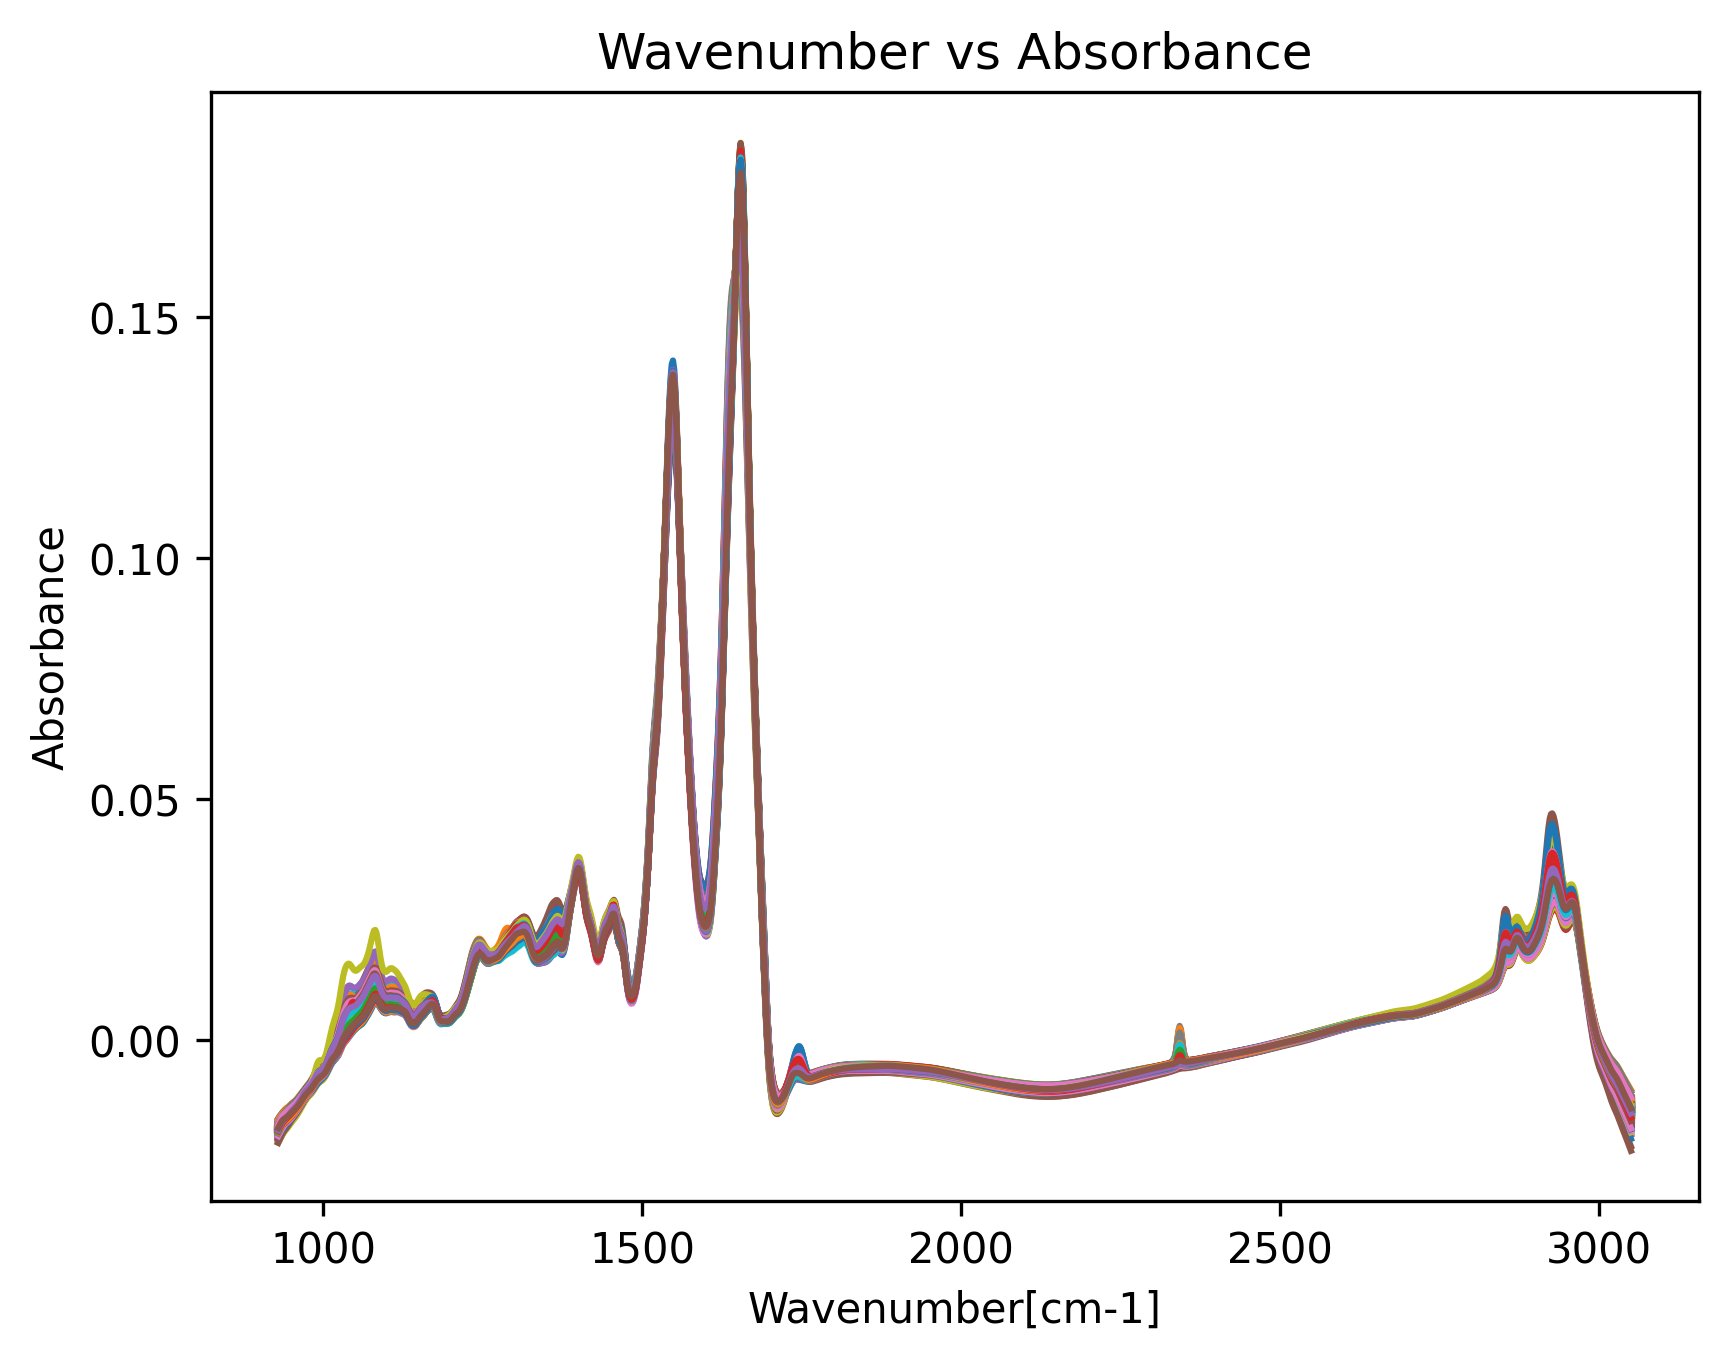
\includegraphics[width=0.9\linewidth]{images/Lung_FTIR.png}
    \caption{Normalised spectra of Lung FTIR data (no water processing was done)}
    \label{FTIR_Spectra}
\end{figure}

\begin{figure}[h!]
    \centering
    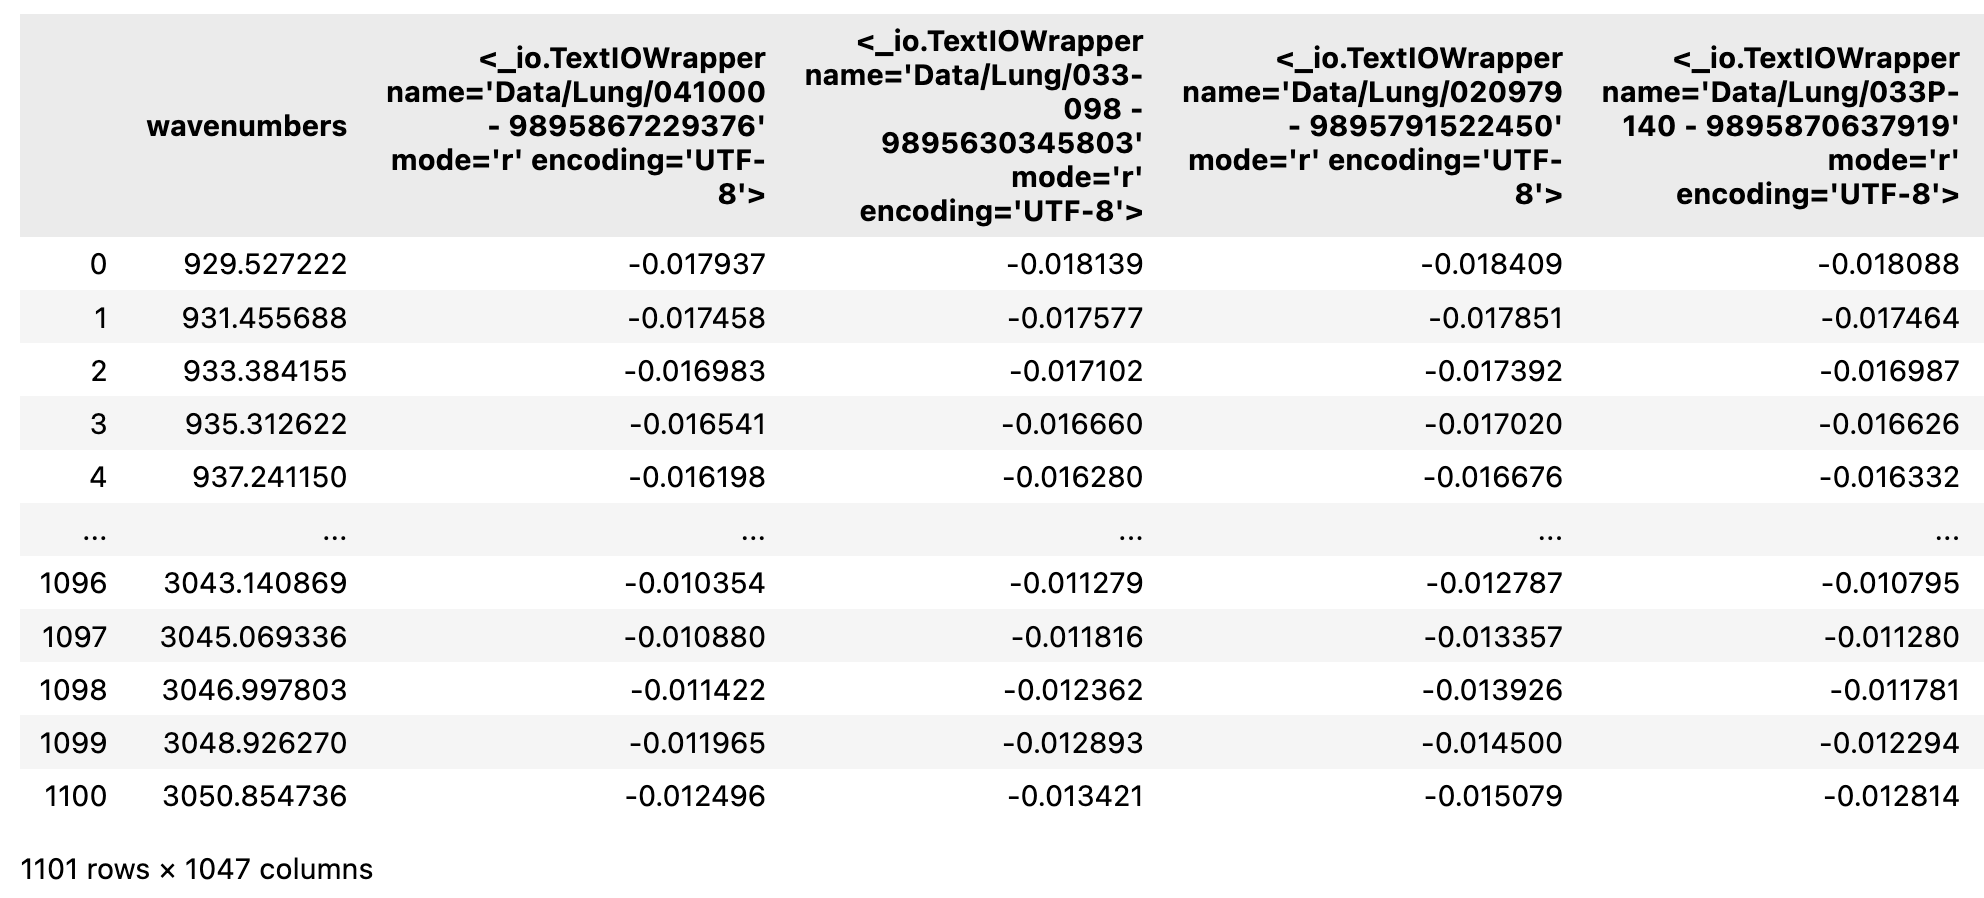
\includegraphics[width=1\linewidth]{images/DataStructure.png}
    \caption{Structured data: The first column represents the serial number of row, second is the wavenumbers captured in the spectra, and the next columns represent the spectral data sets. The dimension of our dataframe is $1101\times1047$.}
    \label{Data}
\end{figure}









\newpage
\subsection{Differential fingerprint and Principle component analysis}

For this section the code can be found in the file difference\_curves.ipynb. The code can be described as follows:

\begin{enumerate}

\item \textbf{Import Necessary Libraries:} Several more libraries were imported for this part of the analysis, including Matplotlib for data visualization, Seaborn for statistical data visualization, and sklearn.decomposition for performing Principal Component Analysis (PCA).

\item \textbf{Load the Data:} Our training data was loaded from the CSV file 'training\_data.csv'. The spectral data was extracted and converted into a numpy array for easier manipulation. The labels corresponding to each spectrum were also extracted and stored in a numpy array.

\item \textbf{Separate Spectra Based on Labels:} The spectra were separated based on their corresponding labels into two groups: healthy and cancerous. This was accomplished using a simple for loop that iterated over the labels and placed each spectrum into the appropriate group.

\item \textbf{Calculate Average Spectra:} For each group (healthy and cancerous), we calculated the average spectra. This was achieved by taking the mean of the spectra along the zeroth axis (i.e., averaging over all individual spectra). We also calculated the average difference between the cancerous and healthy spectra.

\item \textbf{Load Wavenumbers:} The wavenumbers corresponding to each point in the spectra were loaded from the 'combined\_data.csv' file.

\item \textbf{Plot Average Difference:} A plot was made showing the average difference between the healthy and cancerous spectra as a function of wavenumber. This provided a visual representation of how the average spectra of the two groups differ (refer fig.\ref{DF}). It can be seen that the most prominent lung cancer features are in the range 1500-1750 $cm^-1$.  

\item \textbf{Perform PCA and Visualize Results:} PCA was performed on the spectral data to reduce its dimensionality and visualize it in a 2D scatter plot \cite{PCA}. The first two principal components were plotted against each other, with data points colored based on their labels (healthy vs. cancerous). This plot assisted in visualizing the separability of the spectra based on their labels in the reduced dimensional space (refer fig.\ref{PCA}).
\end{enumerate}


\begin{figure}[h!]
    \centering
    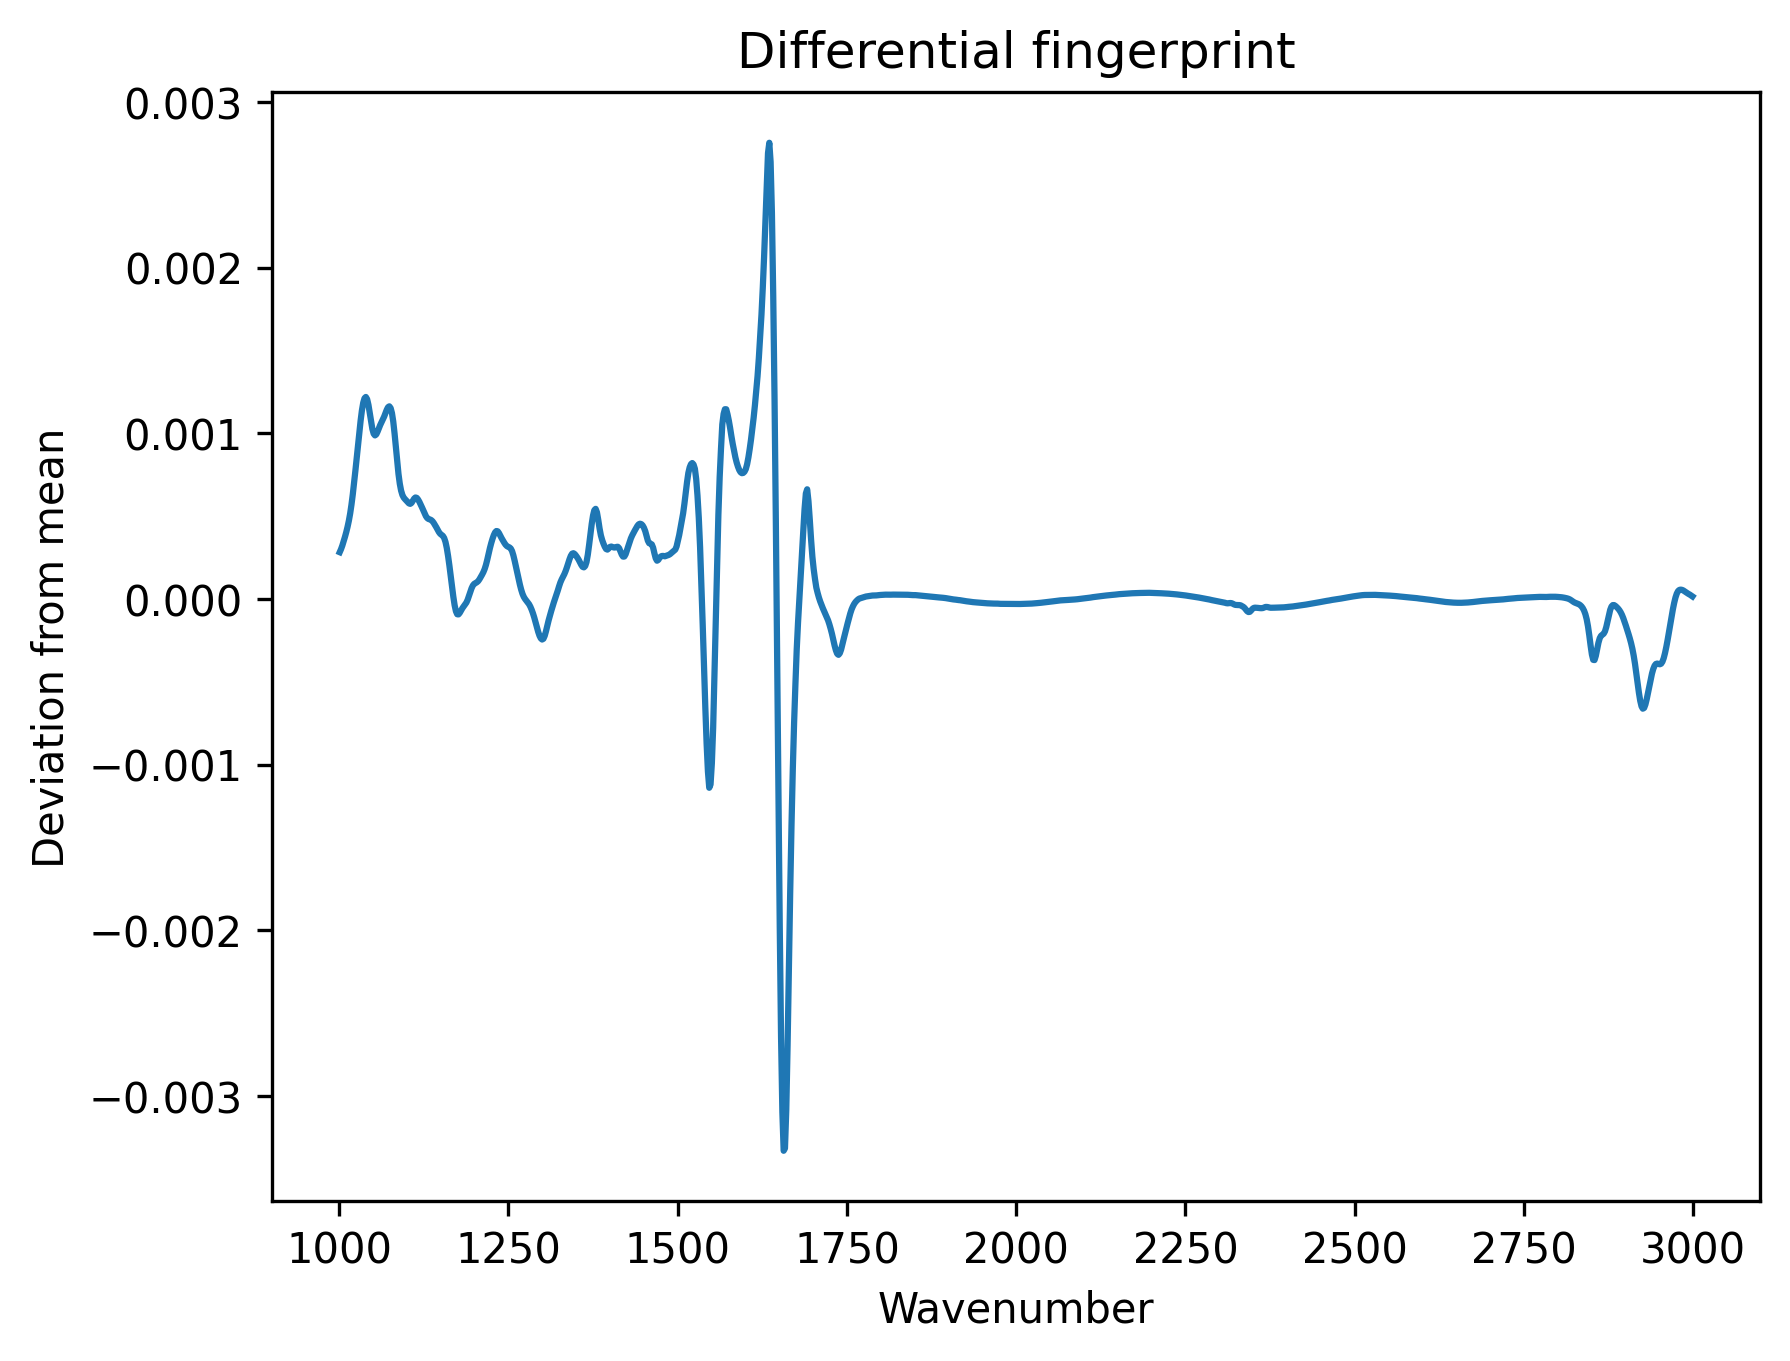
\includegraphics[width=1\linewidth]{images/DF.png}
    \caption{Differential fingerprint (mean of cases minus mean of controls). This plot visulaises the difference between the healthy and cancerous spectra.}
    \label{DF}
\end{figure}


\begin{figure}[h!]
    \centering
    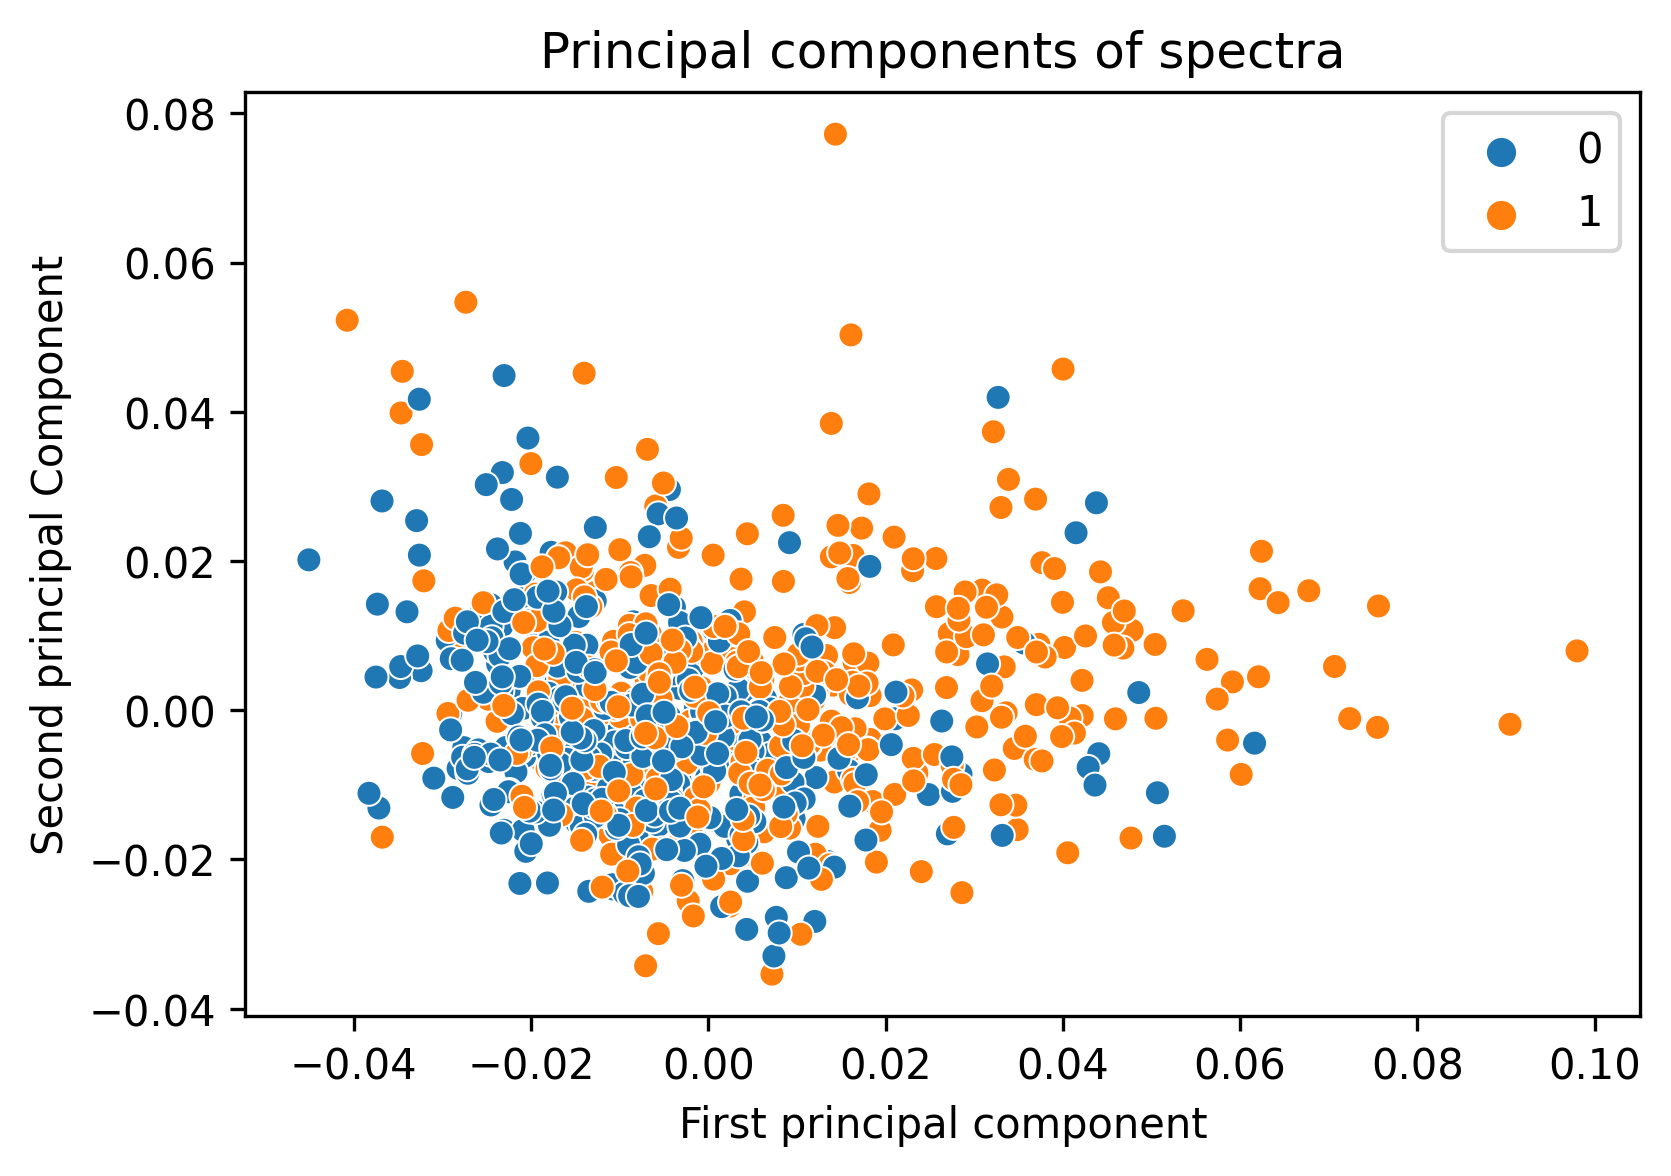
\includegraphics[width=1\linewidth]{images/PCA.png}
    \caption{Scatter plot of the first two principal components. It visualizes the separability of the spectra based on their labels in the reduced dimensional space.}
    \label{PCA}
\end{figure}












\newpage
\subsection{Training and testing the SVM/Logistic regression models}

\begin{figure}
    \centering
    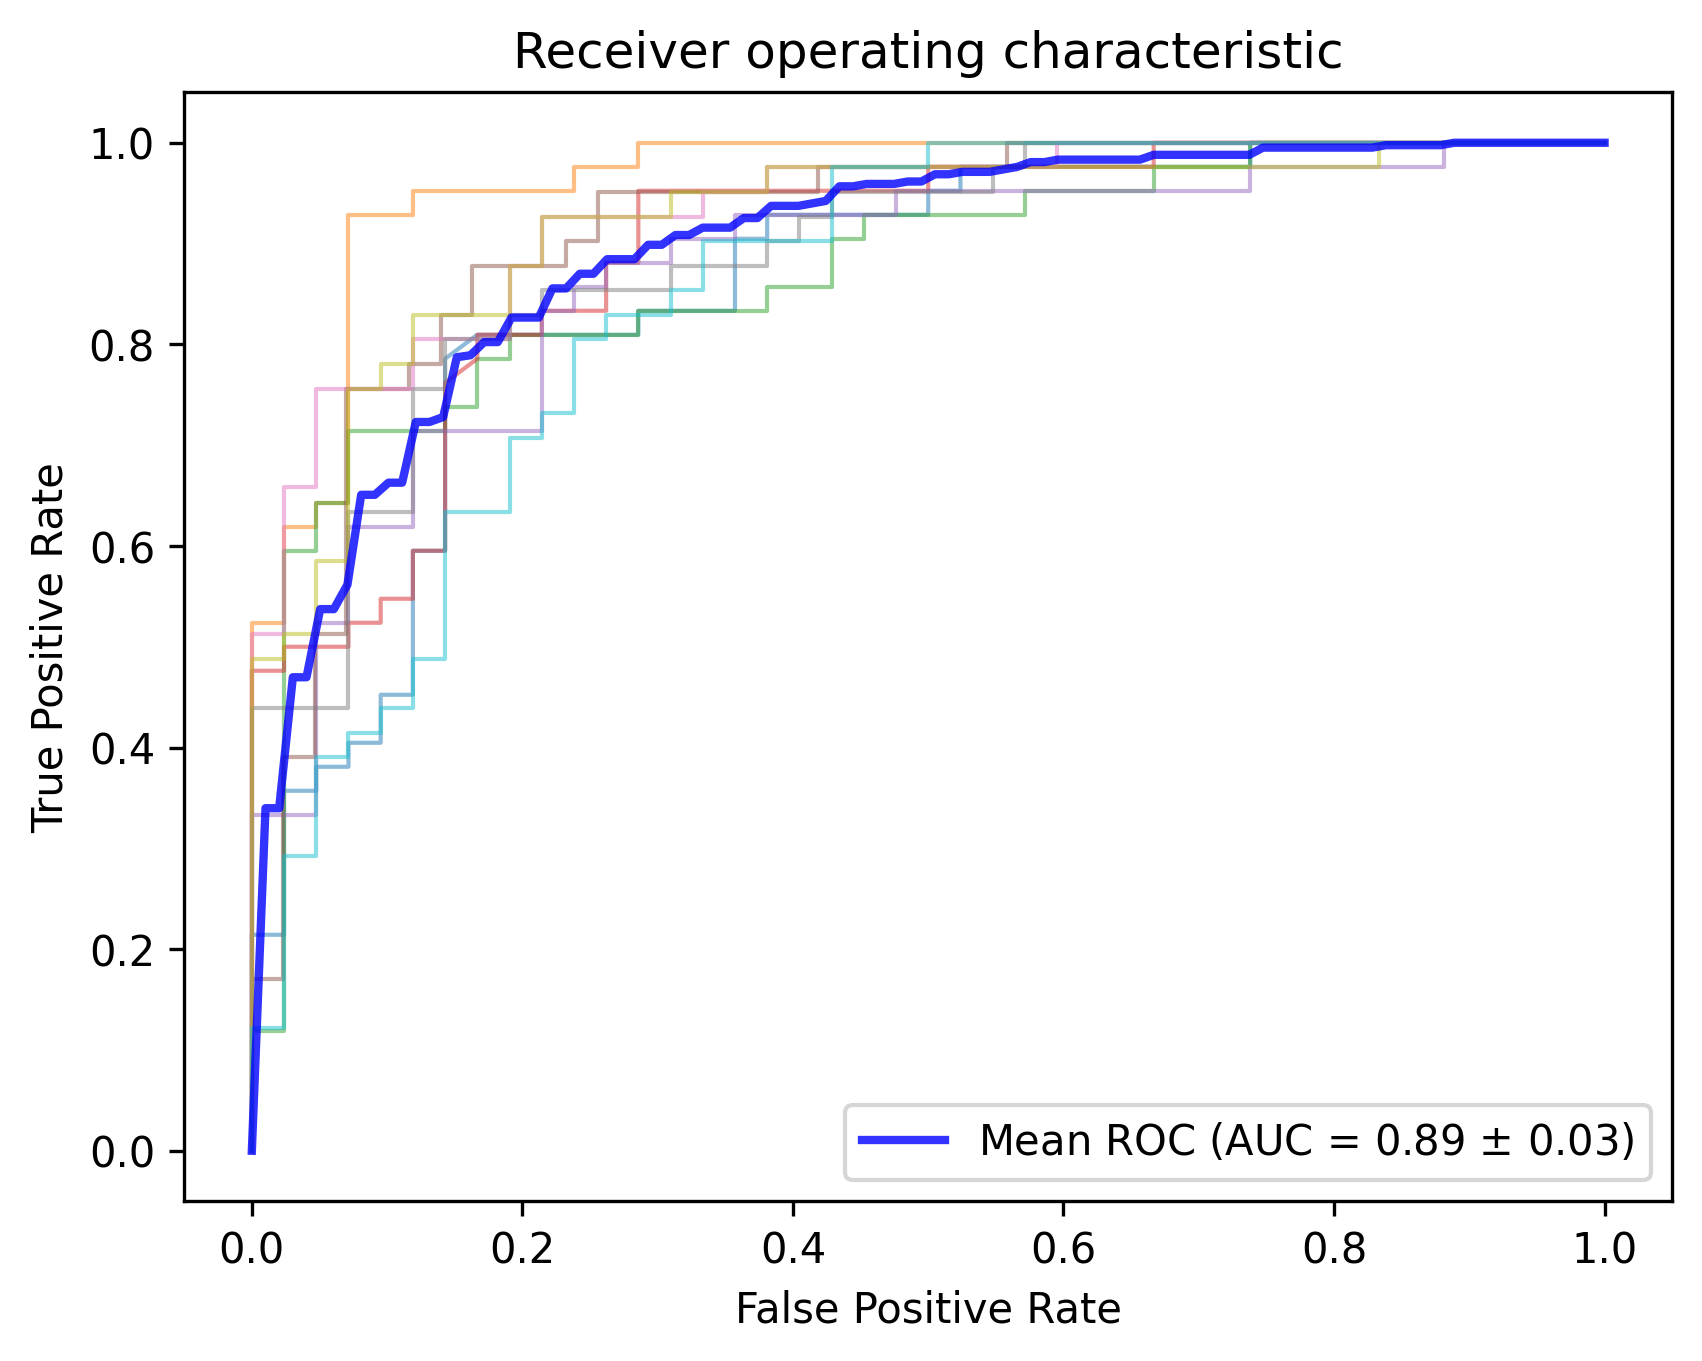
\includegraphics[width=0.8\linewidth]{images/ROC_training_SVM.png}
    \caption{ROC(Receiver operating characteristic) of support vector machine on the training data}
    \label{ROC_training_SVM}
\end{figure}


\begin{figure}
    \centering
    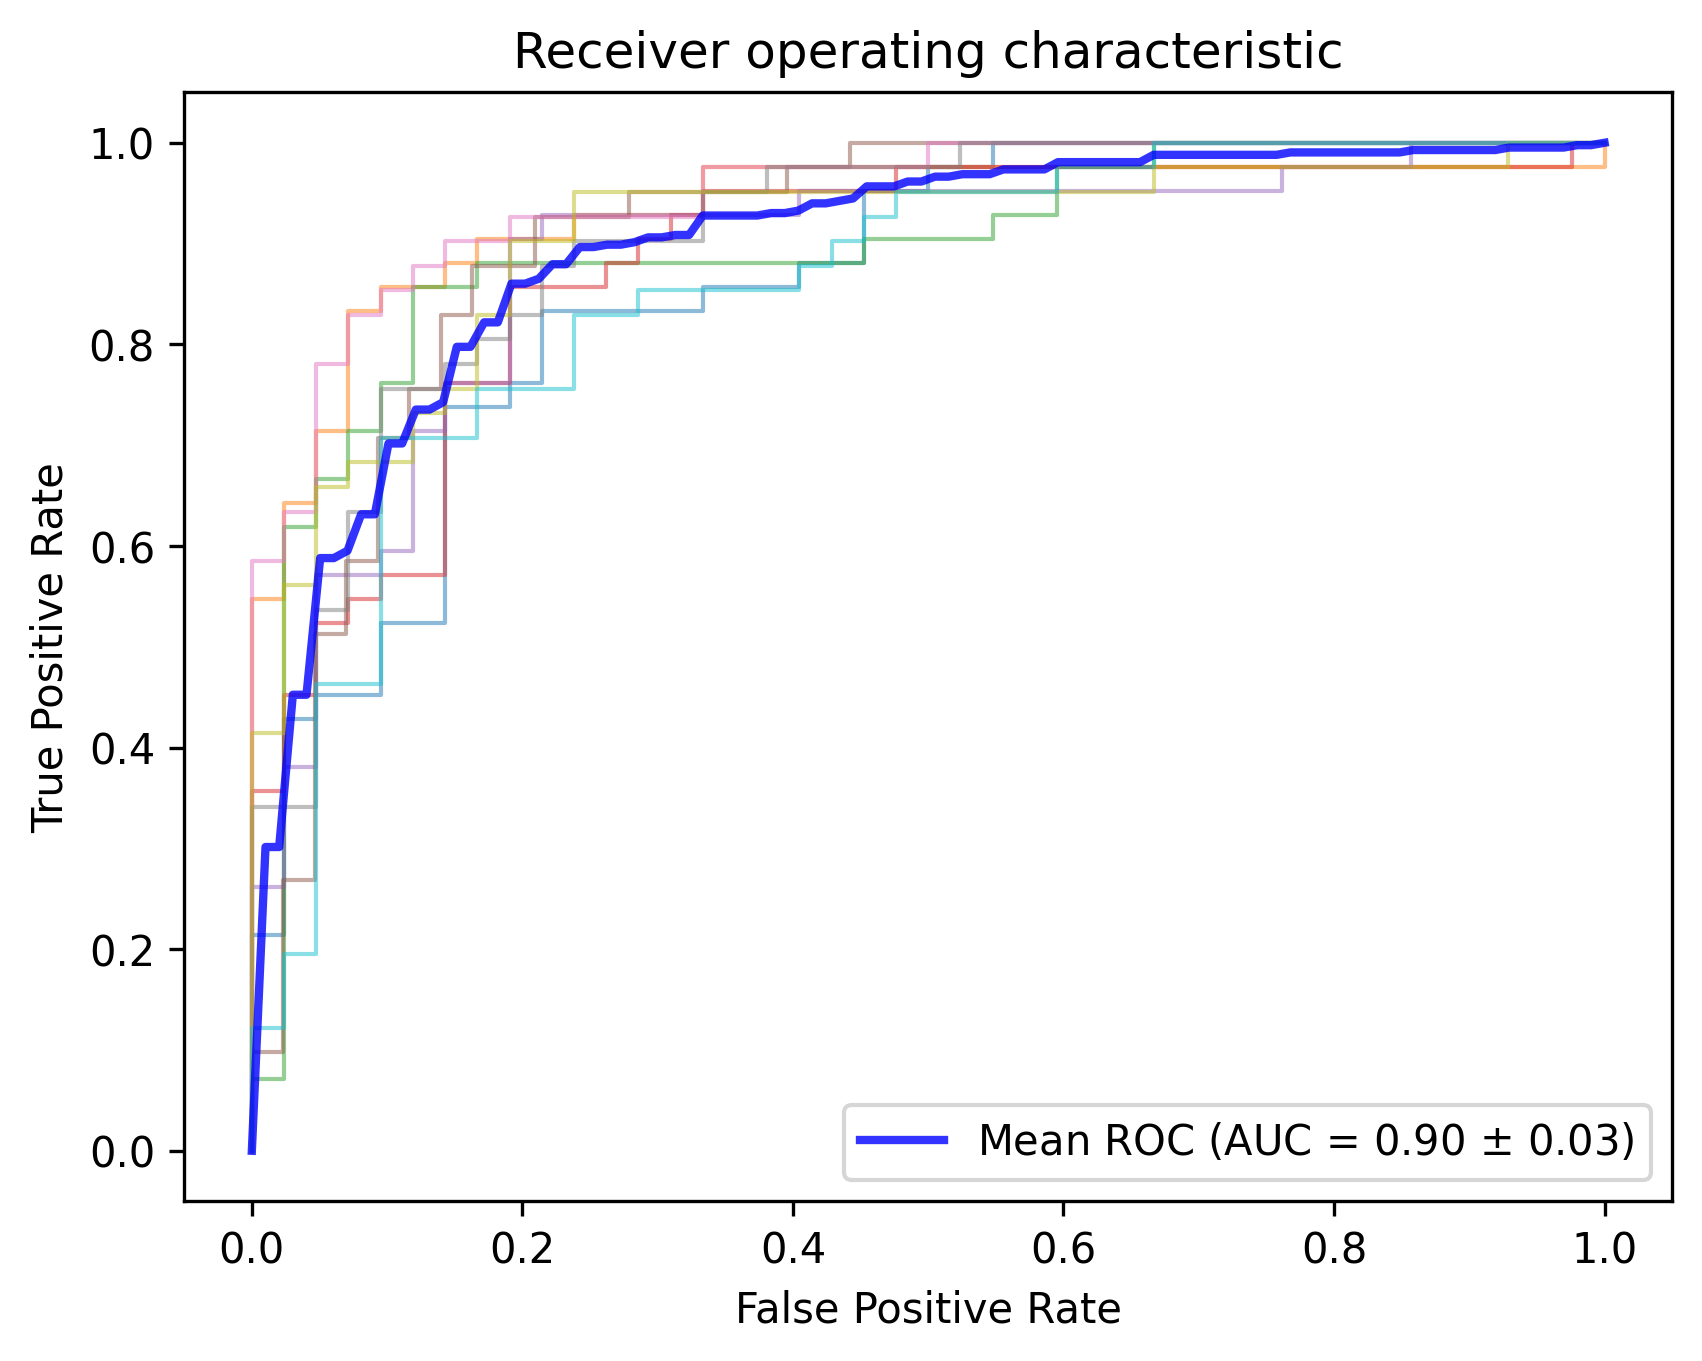
\includegraphics[width=0.8\linewidth]{images/ROC_training_lreg.png}
    \caption{ROC(Receiver operating characteristic) of logistic regression on the training data}
    \label{ROC_training_lreg}
\end{figure}


\begin{figure}
    \centering
    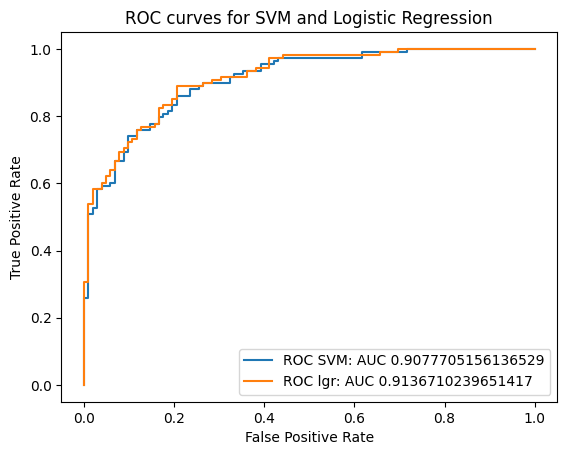
\includegraphics[width=0.8\linewidth]{images/ROC_test_SVM_and_lreg.png}
    \caption{Comparison of ROC(Receiver operating characteristic), AUC(Area under the curve) of support vector machine and logistic regression on the test data}
    \label{ROC_test_SVM_and_lreg}
\end{figure}

For this section the code can be found in the files svm\_lreg\_training.ipynb and\\ svm\_lreg\_test.ipynb. The code can be described as follows:

\begin{enumerate}
\item \textbf{Import Necessary Libraries:} We imported additional libraries necessary for the construction and evaluation of our ML models. These libraries include \texttt{svm} and \texttt{LogisticRegression} for the ML models, \texttt{train\_test\_split}, \texttt{cross\_val\_score},\\ \texttt{GridSearchCV}, \texttt{StratifiedKFold}, and \texttt{RepeatedStratifiedKFold} for data splitting and parameter tuning, \texttt{Pipeline} for constructing ML pipelines, \texttt{roc\_curve}, \texttt{auc}, and \texttt{roc\_auc\_score} for model evaluation, and \texttt{pickle} for saving and loading models.

\item \textbf{Load the Training Data:} Similar to the previous phase, we loaded our training data from the CSV file 'training\_data.csv', extracted the spectral data, and converted it into a numpy array.


\item \textbf{Construct and Evaluate LR, SVM Models:} We constructed a pipeline for the LR model that includes standard scaling of features and the LR model itself. we used Logistic Regression and Support Vector Machine (SVM) as the machine learning models for binary classification. To optimize these models and evaluate their performance, we adopted a nested cross-validation scheme with stratified k-fold cross-validation for both the inner and outer loops. We chose this scheme to ensure a robust estimate of the model's performance and to prevent overfitting. The outer loop was used for validating the model's performance, while the inner loop was used for hyperparameter tuning. We set the number of folds in the outer loop to 10 and the inner loop to 5, providing a good balance between bias and variance in our model performance estimates.

For the Logistic Regression model, we created a pipeline that first standardized the features using StandardScaler and then applied the Logistic Regression model. The regularization strength of the Logistic Regression model was optimized over a grid of values [0.1,1,10,100], specified by the parameter 'C'. The 'l2' penalty was used for regularization, which helps prevent overfitting by adding a penalty for complexity to the loss function.

For the SVM model, we followed a similar procedure. The pipeline for the SVM model first standardized the features and then applied the SVM model. The hyperparameters of the SVM model were tuned over a grid of values. The 'C' parameter represents the penalty parameter of the error term, determining the trade-off between achieving a low training error and a low testing error. The 'kernel' parameter was set to 'linear', indicating the use of a linear kernel function. The 'gamma', 'coef0', 'degree' parameters are not used by the linear kernel. We evaluated the model using the area under the ROC curve (AUC).

\item \textbf{Construct and Evaluate SVM Model:} Similarly, we constructed a pipeline for the SVM model, performed hyperparameter tuning, and evaluated the model using the AUC. The performance of the model was visualized through a ROC curve.

\item \textbf{Load the Testing Data:} We loaded our testing data from the CSV file 'testing\_data.csv', extracted the spectral data and the labels, and converted them into numpy arrays.

\item \textbf{Evaluate the Models on the Testing Data:} We evaluated both the SVM and LR models on the testing data. The models' performances were visualized through ROC curves, and the AUC was computed (refer fig.\ref{ROC_training_SVM}, \ref{ROC_training_lreg}). It can be seen that the logistic regression model scored higher (AUC=0.90) compared to SVM's 0.89 both with a standard deviation of 0.03.

\item \textbf{Evaluating and Comparing the SVM, Logistic Regression on test dataset}
Both the SVM, logistic regression models, previously saved after training, are loaded and used to predict the labels of the test data. The \texttt{GridSearchCV} function from scikit-learn is used to optimize the hyperparameters. The model is evaluated based on the Area Under the Receiver Operating Characteristic (ROC) Curve (AUC). The ROC curves are plotted for both models and the optimal points on the ROC curve is calculated and printed. The ROC curves for both the SVM and Logistic Regression models are plotted on the same graph for comparison (refer fig.\ref{ROC_test_SVM_and_lreg}). Again, logistic regression's AUC is higher (0.91) compared to SVM's 0.90.


\item \textbf{Computing the Optimal Point:} We computed the "optimal point" on the Receiver Operating Characteristic (ROC) curve for the logistic regression model. The optimal point on an ROC curve is usually considered the point closest to the top-left corner of the plot (i.e., the point with the highest true positive rate (TPR) and the lowest false positive rate (FPR)). We calculated the Euclidean distance from each point on the ROC curve to the top-left corner of the plot (0,1), and found the point with the smallest distance. The Euclidean distance is calculated as \(\sqrt{(1 - \text{{TPR}})^2 + (\text{{FPR}})^2}\), which is minimized when the TPR is high and the FPR is low. We then printed the FPR and TPR values of the optimal point. This optimal point provides a single, summary measure of the ROC curve and is often used to compare different classifiers. We found the following:\\
Optimal point SVM: (0.20588235294117646, 0.8611111111111112)\\
Optimal point Logistic Regression: (0.20588235294117646, 0.8888888888888888)

\end{enumerate}










\vspace{100cm}
\section{Discussion and Summary}

This experiment involved a series of steps, beginning with the import and preprocessing of FTIR spectroscopy data. We conducted exploratory data analysis, including plotting the mean spectrum of cases and controls and the differential fingerprint. Principal Component Analysis (PCA) was employed for unsupervised analysis, with the resulting scatter-plots aiding in the visualization of data structure. 

We trained Logistic Regression, Support Vector Machines (SVM) models using nested cross-validation. This approach allowed us to use the inner part of the cross-validation for hyperparameter tuning and the outer part for obtaining validation results in the form of Receiver Operating Characteristic (ROC) curves.

In our experiment, we observed that the Logistic Regression model outperformed the Support Vector Machine model in terms of AUC on both the training and testing datasets in terms of AUC and optimal point(FPR, TPR) values. The training time was significantly less with LR(40.6s) compared to SVM's 10min15s. The summarised results are in table \ref{results}. The differences can be attributed to several factors related to the nature of the models and the specific characteristics of our dataset.

\begin{enumerate}
\item \textbf{Model Complexity:} Logistic Regression is a simpler model compared to SVM. The simplicity of Logistic Regression makes it less prone to overfitting, which might have contributed to its superior performance on the testing dataset especially considering that the dataset was binary.

\item \textbf{Assumption about Data:} Logistic Regression makes fewer assumptions about the data distribution compared to SVM. While SVM relies on the data being separable in a transformed feature space, Logistic Regression merely assumes a linear relationship between the feature variables and the log-odds of the response variable. This difference can make Logistic Regression more robust under certain circumstances.

\item \textbf{Feature Importance:} Logistic Regression provides a direct probabilistic framework and allows for the interpretation of feature importance via the coefficients in the model. This means that it can perform well even if some features are irrelevant or slightly harmful. On the other hand, SVM depends more heavily on the selection of the right features and the right kernel to achieve good performance.

\item \textbf{Outliers:} Logistic Regression can be more robust to outliers in the dataset. In SVM, the decision boundary is entirely determined by the support vectors, which are the instances lying on the margin or on the wrong side of the margin. Therefore, SVM can be sensitive to outliers. On the other hand, Logistic Regression is less influenced by outliers as it considers all instances when learning the model parameters.
\end{enumerate}

It is important to note that while Logistic Regression outperformed SVM in our specific case, this does not mean it will always be the superior choice. The best model can vary depending on the specific dataset and task at hand. Therefore, it is always a good practice to try multiple models and select the one that performs best on a validation set. 

Our SVM result on the test data is very close to the results of this study(\cite{huber2021infrared}). We got an AUC of 0.90 compared to their 0.89. We attribute this difference to pre-processing since we did not implement water correction on the spectral data, hence the slight overestimation. In all, our result serves as strong evidence supporting the validity and quality of our study. 

In summary, the ROC curves and corresponding AUCs highlight the potential of machine learning methodologies using binary classification in disease diagnostics based on FTIR spectroscopy data.

\begin{table}[h]
\centering
\caption{Performance Comparison of Logistic Regression and SVM \footnotemark}
\begin{tabular}{|c|c|c|c|c|c|}
\hline
\textbf{Model} & \textbf{AUC (Test)} & \textbf{AUC (Train)} & \textbf{Std. Dev.} & \textbf{Optimal Point} & \textbf{Training Runtime} \\
\hline
SVM & 0.90 & 0.89 & 0.03 & (0.2059, 0.8611) & 10min 15s\\
\hline
LR & 0.91 & 0.90 & 0.03 & (0.2059, 0.8889) & 40s \\
\hline
\end{tabular}
\label{results}
\end{table}
\footnotetext{The runtime was obtained by running the models on an M1 pro chip, with 16GB RAM, on MacOS 13.3.1.}



\newpage

\bibliography{references}

\bibliographystyle{plain}

\end{document}